\chapter{Utiliser les ressemblances entre les maladies transmises par {\em Aedes} pour améliorer les outils de prédiction épidémique}
\chaptermark{Prédire}

\section{Guider les interventions de prévention et de contrôle en situation d'épidémie émergente}

\subsection{Approches classiques en prédiction}

\subsection{Récents développements : les challenges}

\section{Améliorer les prédictions à la phase précoce d'une épidémie de Zika grâce aux données historiques sur la transmission du Chikungunya}

\subsection{Résumé de l'article en français}

\subsection{Article : Riou, Poletto, Boëlle, Improving early epidemiological assessment of emerging {\em Aedes}-transmitted epidemics using historical data}
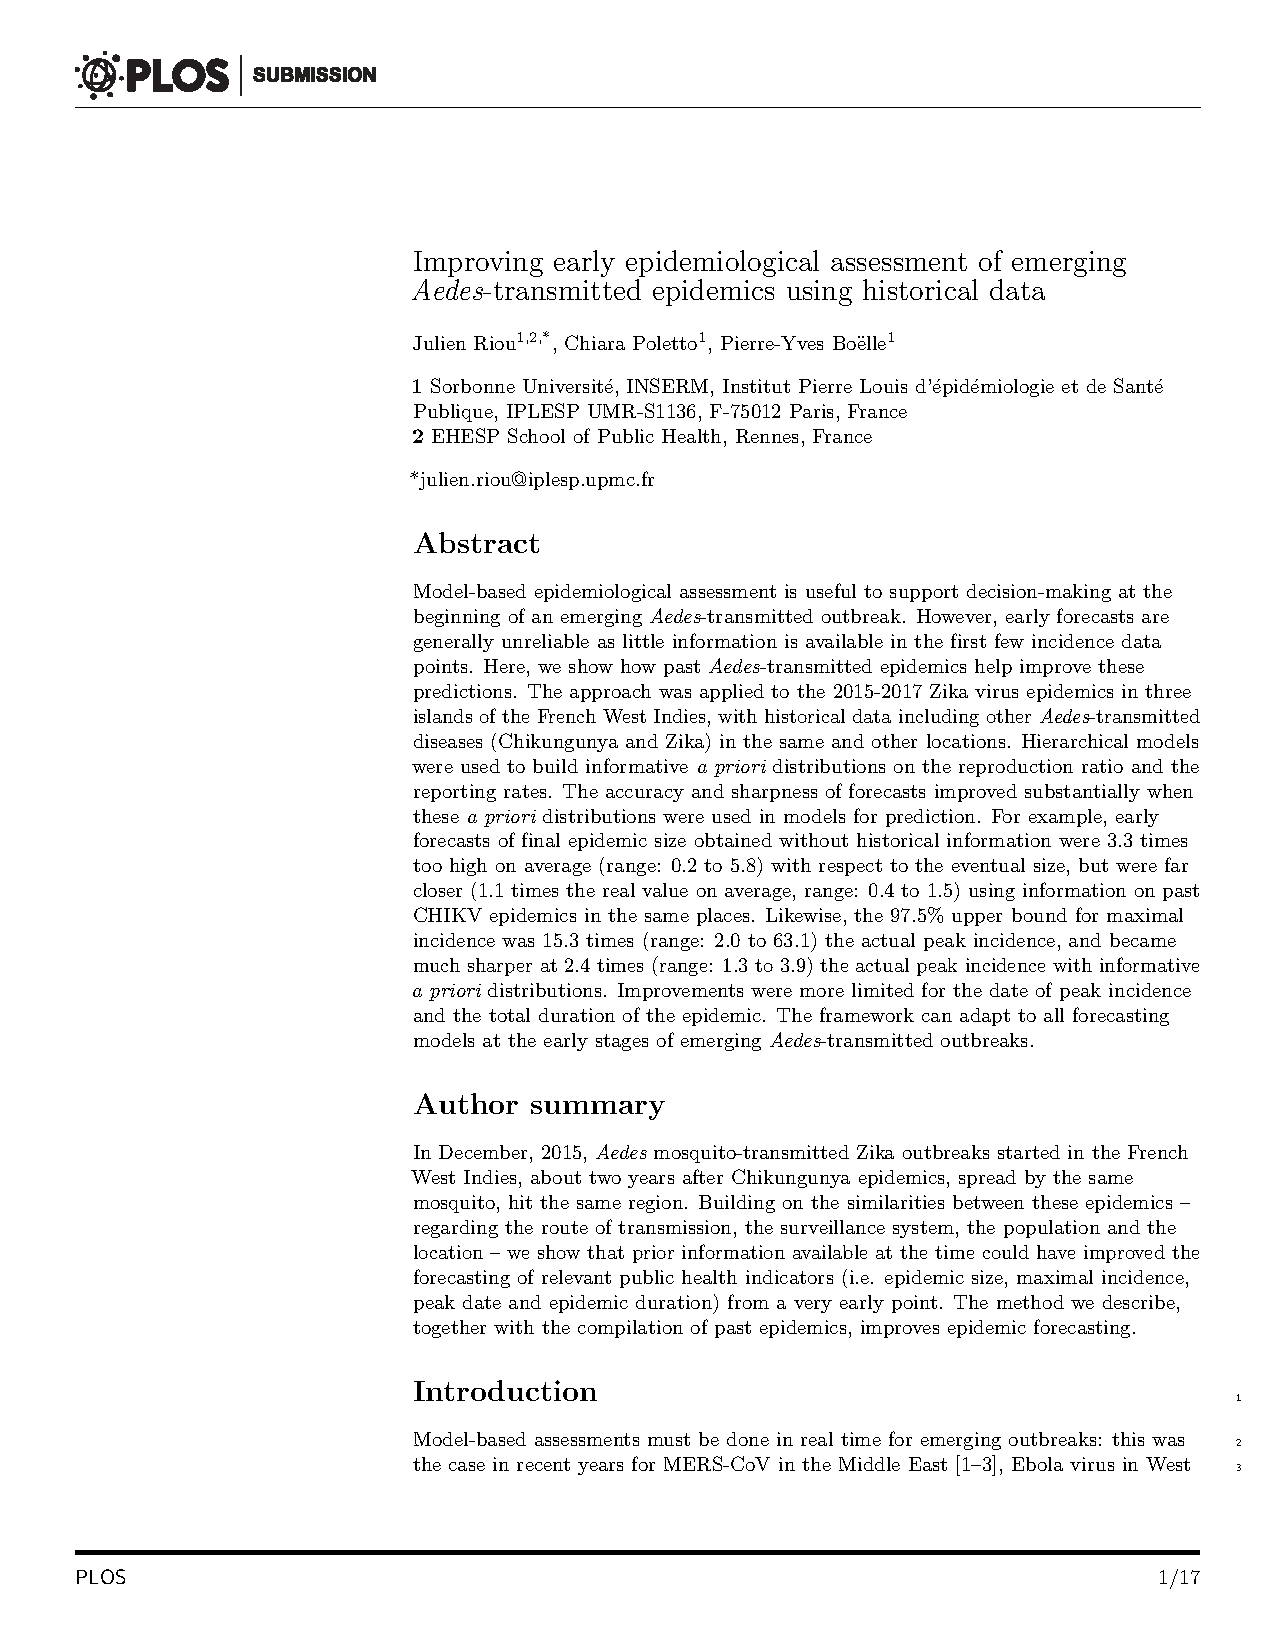
\includepdf[pages={1}]{Articles/Predictionv12.pdf}
%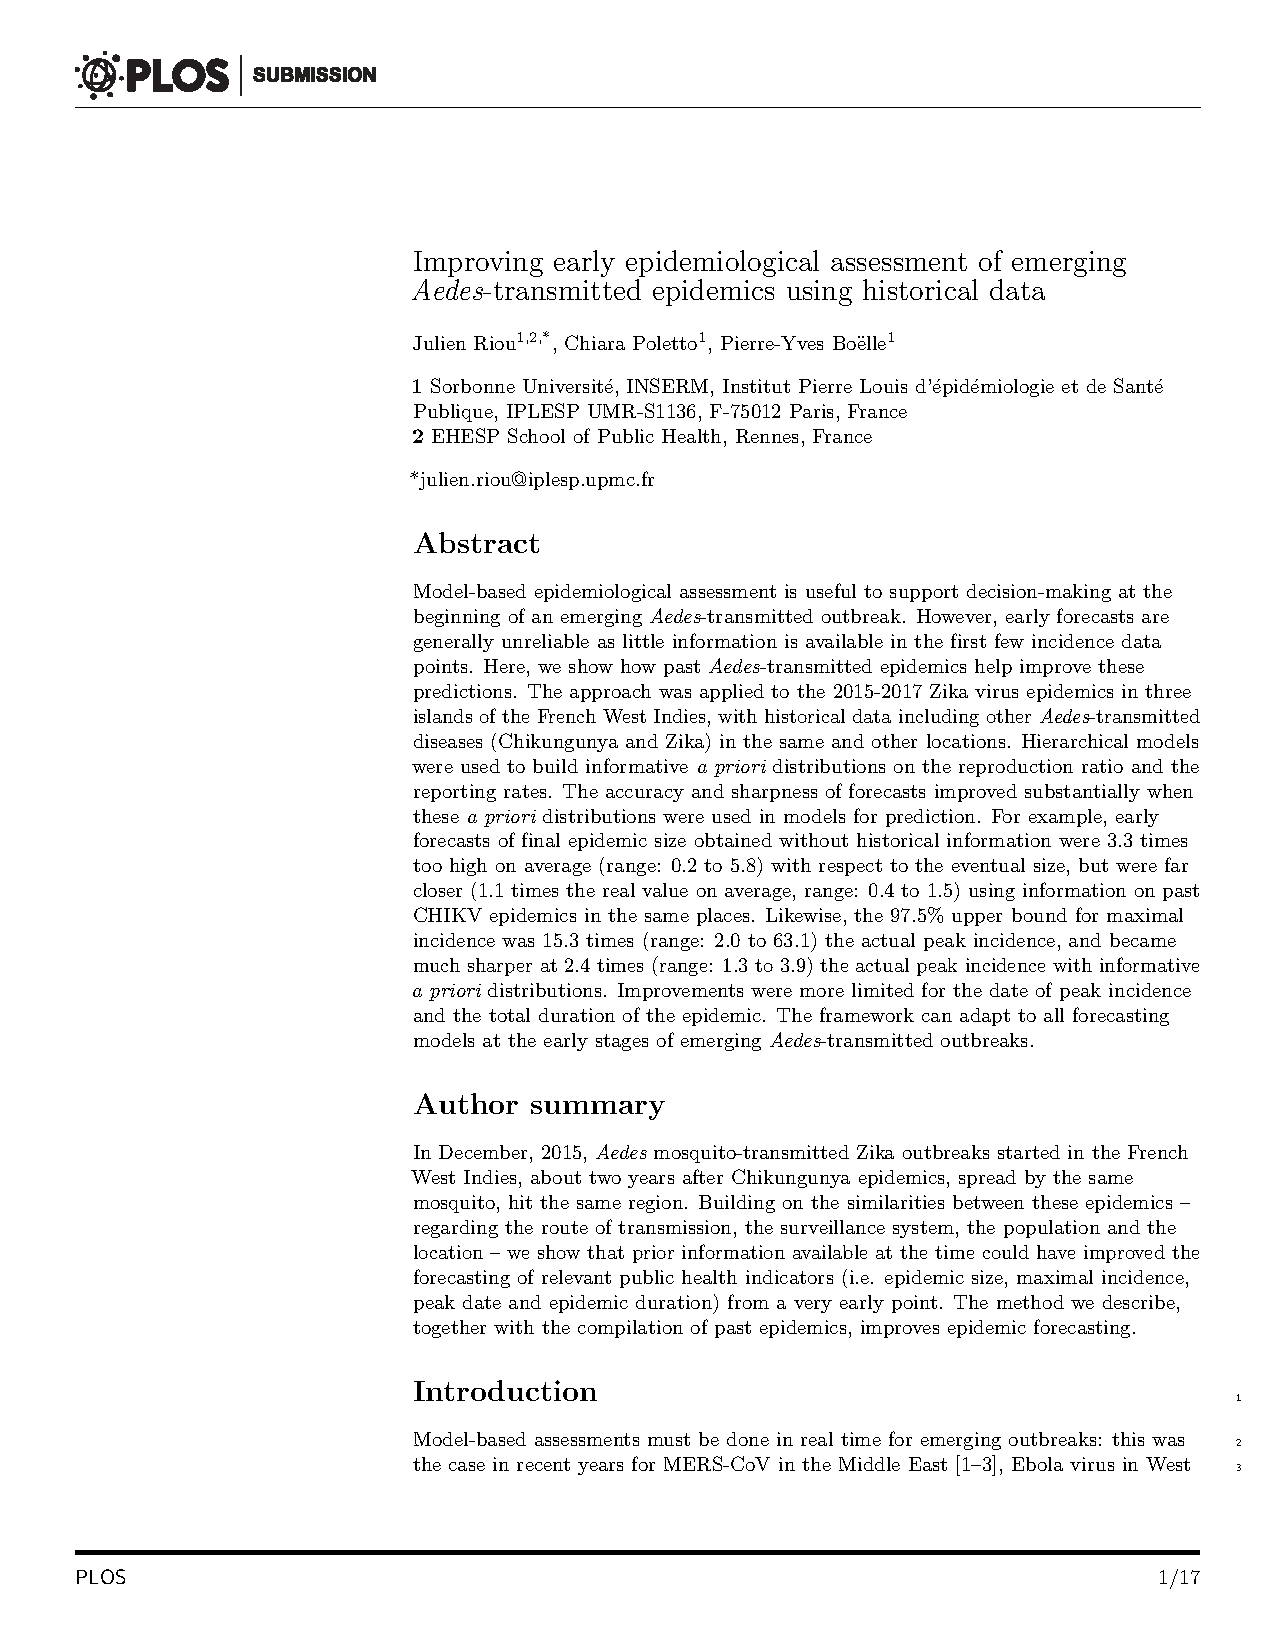
\includepdf[pages={1-17}]{Articles/Predictionv12.pdf}

\section{Commentaires et perspectives}
\sectionmark{ }
